
\begin{figure*}[t]
    \centering
     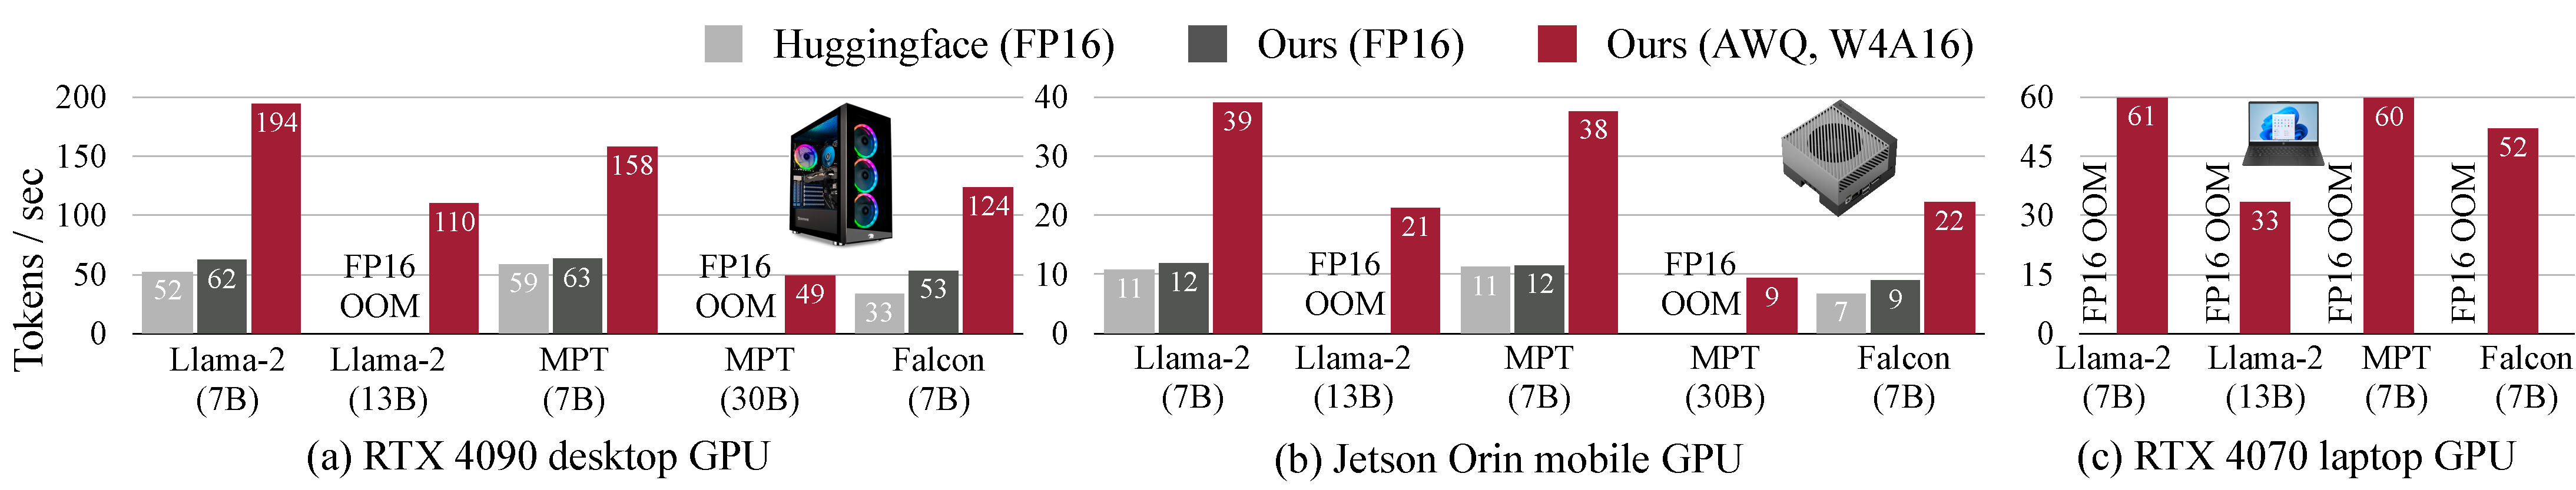
\includegraphics[width=\textwidth]{figures/speedup.pdf}
\caption{\system provides a turn-key solution to transform the theoretical memory footprint reduction into a quantifiable speedup. As a result, \system is up to \textbf{3.9$\times$} and \textbf{3.5$\times$} faster than the FP16 implementation from Huggingface on 4090 (desktop GPU) and Orin (mobile GPU), respectively. AWQ also democratizes Llama-2-13B deployment on laptop GPUs (4070) with merely 8GB memory.} %
    \label{fig:kernel_speedup}
\end{figure*}


\begin{figure*}[t]
    \centering
     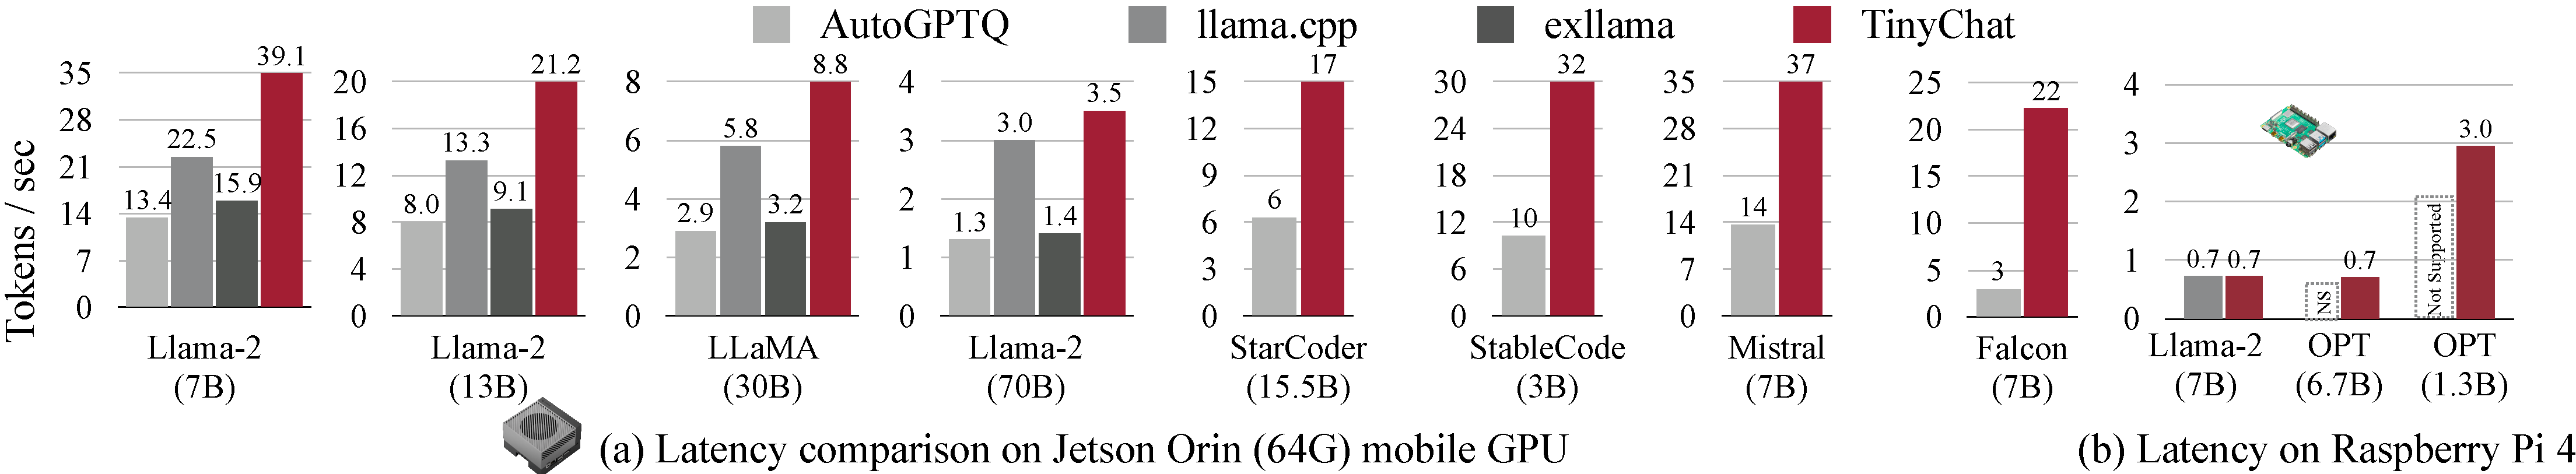
\includegraphics[width=\textwidth]{figures/speedup_comparisons.pdf}
\caption{\system offers \textbf{1.2-3.0$\times$} speedup over existing systems when running 4-bit quantized Llama models on NVIDIA Jetson Orin. It also supports a diverse range of general-purpose and coding-specific LLMs with at least \textbf{2.6$\times$} speedup over AutoGPTQ, which also supports all these workloads. Moreover, \system seamlessly operates on Raspberry Pi and enables the deployment of LLMs with up to 7 billion parameters on extremely resource-constrained IoT devices.} %
    \label{fig:kernel_speedup_comparisons}
\end{figure*}
